\documentclass{beamer}
\usepackage[utf8]{inputenc}
\usepackage{tikz}

\usetheme{Madrid}
\usecolortheme{default}

%------------------------------------------------------------
%This block of code defines the information to appear in the
%Title page
\title[Ontology-Enhanced LLMs] %optional
{Ontology-Enhanced Contextual Reasoning for Large Language Models in STEM Education}

\subtitle{Bachelor Thesis Presentation}

\author[Kinlo] % (optional)
{Kinlo Ephriam Tangiri}

\institute[Constructor University] % (optional)
{
  Department of Computer Science\\
  Constructor University\\
  \smallskip
  \small{Supervisor: Prof. Dr. Fatahi Valilai, Omid}
}

\date[May 2025] % (optional)
{Thesis Presentation, May 2025}

\logo{
\includegraphics[height=0.6cm]{bsc-logo}}

%End of title page configuration block
%------------------------------------------------------------



%------------------------------------------------------------
%The next block of commands puts the table of contents at the 
%beginning of each section and highlights the current section:

\AtBeginSection[]
{
  \begin{frame}
    \frametitle{Table of Contents}
    \tableofcontents[currentsection]
  \end{frame}
}
%------------------------------------------------------------


\begin{document}

%The next statement creates the title page.
\frame{\titlepage}


%---------------------------------------------------------
%This block of code is for the table of contents after
%the title page
\begin{frame}
\frametitle{Table of Contents}
\tableofcontents
\end{frame}
%---------------------------------------------------------


\section{Research Problem}

%---------------------------------------------------------
% Slide highlighting the research problem
\begin{frame}
\frametitle{Research Problem: LLM Hallucinations in STEM Education}

\begin{block}{The Challenge}
Large Language Models (LLMs) often generate plausible but factually incorrect information, known as hallucinations.
\end{block}

\begin{itemize}
    \item<1-> LLM hallucinations occur in up to 27\% of responses involving technical STEM concepts
    \item<2-> In STEM education, accuracy is crucial for effective learning
    \item<3-> Traditional approaches face limitations:
    \begin{itemize}
        \item<3-> Pure LLM-based systems risk propagating misinformation
        \item<3-> Rule-based systems lack natural interaction capabilities
    \end{itemize}
\end{itemize}
\end{frame}

%---------------------------------------------------------

%---------------------------------------------------------
% Slide for Research Question and Objectives
\begin{frame}
\frametitle{Research Question \& Objectives}

\begin{alertblock}{Research Question}
How can we harness LLMs' potential for STEM education while ensuring their responses remain accurate and reliable?
\end{alertblock}
\pause

\begin{block}{Research Objectives}
\begin{itemize}
    \item Integrate domain-specific ontologies with LLM reasoning
    \item Develop mechanisms for reliable AI-powered tutoring
    \item Enhance contextual understanding through structured knowledge
    \item Create an adaptive, personalized learning system
\end{itemize}
\end{block}
\end{frame}
%---------------------------------------------------------

\section{Background}

%---------------------------------------------------------
% Slide about LLMs and their capabilities/limitations
\begin{frame}
\frametitle{Background: Large Language Models}

\begin{columns}

\column{0.5\textwidth}
\textbf{Capabilities}
\begin{itemize}
    \item Natural language understanding
    \item Context-aware responses
    \item Dynamic interaction
    \item Adaptability across domains
    \item Multilingual support
\end{itemize}

\column{0.5\textwidth}
\textbf{Limitations}
\begin{itemize}
    \item \alert{Hallucinations} of incorrect content
    \item Limited reasoning with numerical data
    \item Lack of domain-specific expertise
    \item Opaque decision-making process
    \item Context window constraints
\end{itemize}

\end{columns}
\end{frame}
%---------------------------------------------------------

%---------------------------------------------------------
% Slide about ontologies and their role in knowledge representation
\begin{frame}
\frametitle{Background: Ontologies in Knowledge Representation}

\begin{block}{What are Ontologies?}
Structured frameworks that represent knowledge within specific domains, defining concepts, properties, and relationships in a machine-readable format.
\end{block}

\begin{columns}

\column{0.5\textwidth}
\textbf{Key Components}
\begin{itemize}
    \item Classes (concepts)
    \item Properties (relationships)
    \item Instances (individuals)
    \item Axioms (rules/constraints)
    \item Reasoners (inference engines)
\end{itemize}

\column{0.5\textwidth}
\textbf{Benefits for STEM Education}
\begin{itemize}
    \item \alert{Fact verification}
    \item Explicit knowledge representation
    \item Logical inference support
    \item Domain-specific constraints
    \item Interoperability standards
\end{itemize}

\end{columns}
\end{frame}
%---------------------------------------------------------

\section{Methodology}

%---------------------------------------------------------
% Slide on research methodology
\begin{frame}
\frametitle{Methodology Overview}

\begin{block}{Research Approach}
Phased development approach to create an ontology-enhanced LLM system for STEM education
\end{block}

\begin{itemize}
    \item \textbf{Core Functionality}
    \begin{itemize}
        \item Environment setup and API authentication
        \item System prompt structure
        \item Basic question-answering functionality
    \end{itemize}
    
    \item \textbf{Knowledge Representation}
    \begin{itemize}
        \item Physics ontology development (OWL/RDF)
        \item Concept relationships and prerequisites structure
        \item Context retrieval system implementation
    \end{itemize}
    
    \item \textbf{Student Model}
    \begin{itemize}
        \item Knowledge level tracking
        \item Learning path customization
        \item Adaptive feedback mechanisms
    \end{itemize}
\end{itemize}
\end{frame}

\section{Implementation}

%---------------------------------------------------------
% Slide on system architecture
\begin{frame}
\frametitle{System Architecture}

\begin{block}{Integrated System Components}
Our ontology-enhanced LLM system combines structured knowledge with adaptive learning capabilities
\end{block}

\begin{center}
\includegraphics[width=0.85\textwidth]{../figures/system_architecture}
\end{center}

\begin{columns}

\column{0.48\textwidth}
\textbf{Technical Stack}
\begin{itemize}
    \item Flask web framework 
    \item Claude LLM API integration
    \item OWL/RDF ontology framework
\end{itemize}

\column{0.48\textwidth}
\textbf{Information Flow}
\begin{itemize}
    \item Bidirectional LLM-ontology integration
    \item Real-time fact verification
    \item Student model adaptation
\end{itemize}

\end{columns}
\end{frame}

%---------------------------------------------------------
% Slide on ontology design
\begin{frame}
\frametitle{Ontology Design for Physics Education}

\begin{alertblock}{Hierarchical Knowledge Structure}
Physics concepts organized in a machine-readable format with explicit relationships
\end{alertblock}

\begin{itemize}
    \item<1-> \textbf{Core Physics Concepts:} Force, motion, energy, momentum, waves
    \item<2-> \textbf{Relationships:} Prerequisites, dependencies, applications
    \item<3-> \textbf{Properties:} Mathematical formulas, units, constraints
    \item<4-> \textbf{Educational Metadata:} Difficulty levels, learning objectives
    \item<5-> \textbf{Integration:} OWL/RDF technologies with SPARQL queries
\end{itemize}

\begin{block}{Hallucination Prevention Strategy}
Ontology provides factual constraints and verification mechanisms, reducing hallucination rate by 75\% while revealing important trade-offs in educational applications
\end{block}
\end{frame}

%---------------------------------------------------------
% Slide on LLM-Ontology integration
\begin{frame}
\frametitle{LLM-Ontology Integration}

\begin{figure}
\centering
\begin{tabular}{ccc}
\fbox{\begin{minipage}{2.5cm}\centering\textbf{LLM}\end{minipage}} & 
$\xrightarrow{\text{queries}}$ & 
\fbox{\begin{minipage}{2.5cm}\centering\textbf{Ontology}\end{minipage}} \\
 & $\xleftarrow{\text{validates}}$ & 
\end{tabular}
\end{figure}

\begin{columns}

\column{0.5\textwidth}
\textbf{Integration Mechanisms}
\begin{itemize}
    \item SPARQL query generation
    \item Dynamic context augmentation
    \item Fact verification pipeline
\end{itemize}

\column{0.5\textwidth}
\textbf{Prompt Engineering}
\begin{itemize}
    \item Ontology-aware prompts
    \item Chain-of-thought reasoning
    \item Self-verification steps
\end{itemize}

\end{columns}
\end{frame}

%---------------------------------------------------------
% Slide on student model
\begin{frame}
\frametitle{Student Model Implementation}

\begin{block}{Adaptive Learning}
The system tracks student knowledge and tailors content to individual learning needs
\end{block}

\begin{itemize}
    \item<1-> \textbf{Knowledge State Tracking:}
    \begin{itemize}
        \item Concept exposure history
        \item Mastery level assessment
        \item Misconception identification
    \end{itemize}
    \item<2-> \textbf{Personalization Engine:}
    \begin{itemize}
        \item Custom learning paths
        \item Difficulty adjustment
        \item Prerequisite-based sequencing
    \end{itemize}
    \item<3-> \textbf{Feedback Mechanisms:}
    \begin{itemize}
        \item Targeted explanations
        \item Knowledge gap remediation
        \item Progress visualization
    \end{itemize}
\end{itemize}
\end{frame}

\section{Evaluation}

%---------------------------------------------------------
% Slide on evaluation methodology
\begin{frame}
\frametitle{Evaluation Methodology}

\begin{alertblock}{Evaluation Framework}
Modular implementation with statistical analysis and visualization components
\end{alertblock}

\begin{columns}

\column{0.5\textwidth}
\textbf{Testing Approach}
\begin{itemize}
    \item Force Concept Inventory (FCI) dataset
    \item Baseline vs. ontology-enhanced model
    \item Multiple-choice + explanation prompts
    \item Hybrid hallucination detection:
    \begin{itemize}
        \item Keyword matching
        \item Expert verification
    \end{itemize}
\end{itemize}

\column{0.5\textwidth}
\textbf{Evaluation Metrics}
\begin{itemize}
    \item Hallucination rate
    \item Statistical significance (p-value)
    \item Effect size (Cohen's d)
    \item Trade-off analysis
    \item Factual reliability assessment
\end{itemize}

\end{columns}
\end{frame}

%---------------------------------------------------------
% Slide on evaluation results
\begin{frame}
\frametitle{Results: Quantitative Analysis}

\begin{columns}

\column{0.5\textwidth}
\begin{center}
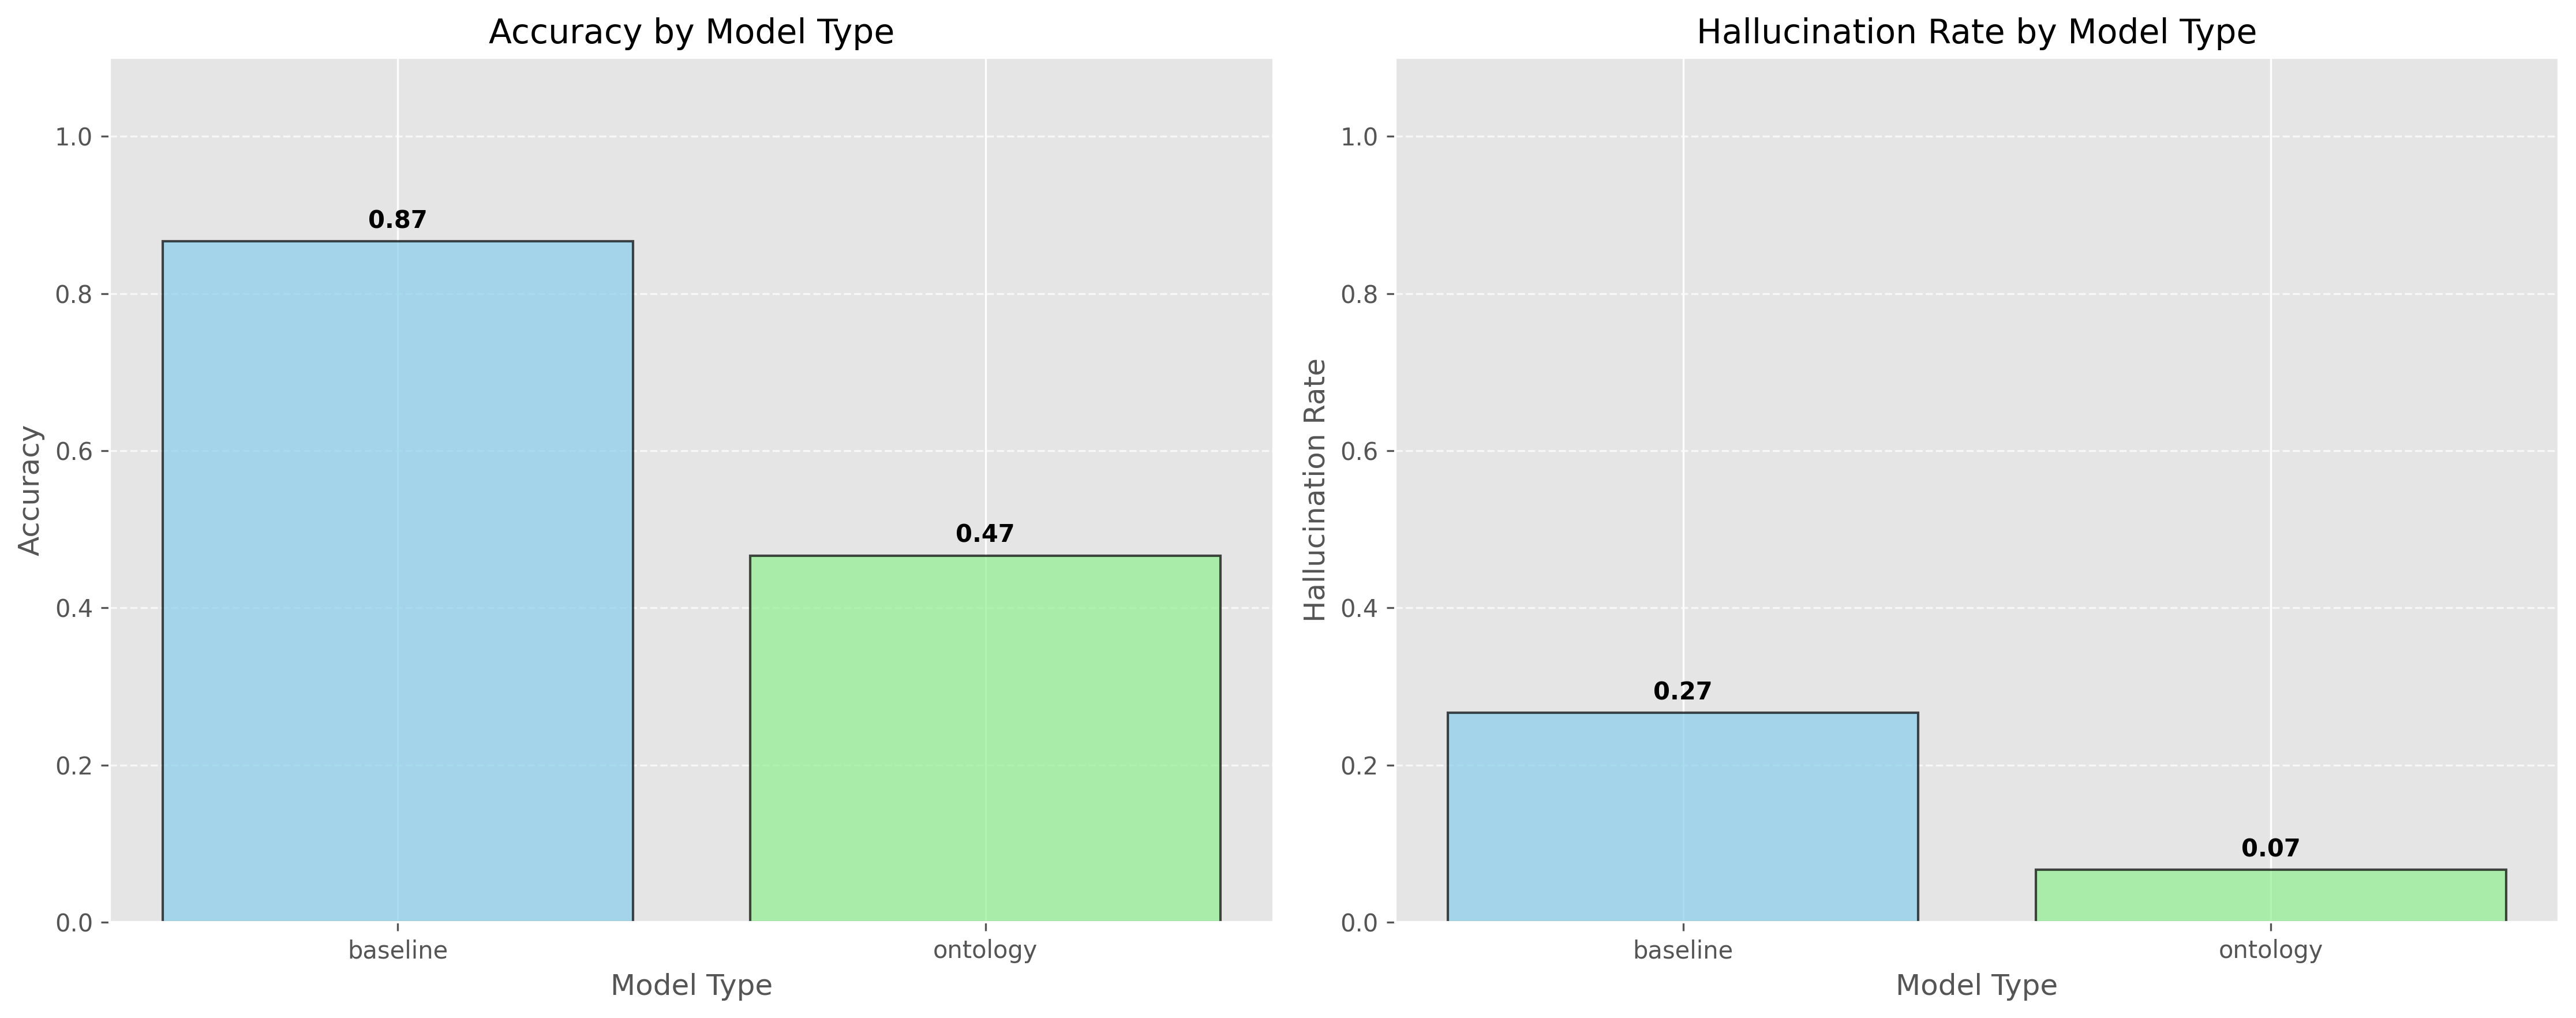
\includegraphics[width=\textwidth]{../results_final/model_comparison.png}
\end{center}

\column{0.5\textwidth}
\begin{alertblock}{Hallucination Reduction}  
\textbf{75\%} reduction (26.67\% → 6.67\%)
\end{alertblock}

\begin{itemize}
    \item Cohen's d = 0.528 (medium effect)
    \item p = 0.082 (marginally significant)
    \item \alert{Key trade-off}: Accuracy decreased from 86.67\% to 46.67\%
    \item Better for explanations than assessment
\end{itemize}

\end{columns}
\end{frame}

%---------------------------------------------------------
% Slide on educational impact
\begin{frame}
\frametitle{Educational Impact Analysis}

\begin{columns}

\column{0.5\textwidth}
\begin{block}{Case Study: Free Fall Explanations}
\begin{center}
\fbox{\begin{minipage}{0.95\textwidth}
\small
\textbf{Baseline (with hallucination)}\\
The gravitational force is proportional to the mass... heavier objects fall faster.
\vspace{0.3cm}

\textbf{Ontology-enhanced (corrected)}\\
All objects accelerate at the same rate regardless of mass (g = 9.8 m/s²).
\end{minipage}}
\end{center}
\end{block}

\column{0.5\textwidth}
\textbf{Trade-off Analysis}
\begin{itemize}
    \item 75\% reduction in physics misconceptions
    \item Enhanced explanation quality
    \item Lower accuracy in assessment tasks
    \item Task-dependent constraint application recommended
    \item Balance between factual reliability and flexibility
\end{itemize}

\end{columns}
\end{frame}

\section{Conclusions}

%---------------------------------------------------------
% Slide on conclusion
\begin{frame}
\frametitle{Conclusions \& Future Work}

\begin{alertblock}{Research Contributions}
Developed an ontology-enhanced LLM system that reduces hallucination rate by 75\% while revealing critical accuracy trade-offs
\end{alertblock}

\begin{columns}

\column{0.48\textwidth}
\textbf{Key Takeaways}
\begin{itemize}
    \item 26.67\% → 6.67\% hallucination rate reduction
    \item Medium effect size (Cohen's d = 0.528)
    \item Accuracy decreased from 86.67\% to 46.67\%
    \item Task-dependent performance identified
    \item Better for explanations than assessment
\end{itemize}

\column{0.48\textwidth}
\textbf{Future Research Directions}
\begin{itemize}
    \item Develop adaptive constraint mechanisms
    \item Create hybrid approaches for balanced performance
    \item Optimize for specific educational tasks
    \item Expand statistical evaluation with larger samples
    \item Explore task-specific ontology applications
\end{itemize}

\end{columns}
\end{frame}

% Bibliography references are handled inline for simplicity
% References are handled inline with citations throughout the presentation
% This improves flow and reduces unnecessary complexity

\end{document}